\section{Modelling}
\begin{figure}[ht]
    \centering
    \begin{minipage}{0.6\textwidth}
        \centering
        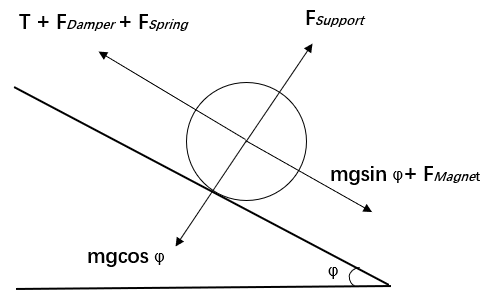
\includegraphics[width=1.20\linewidth]{modelling/Force analysis diagram of the system.png}
        \caption{Force analysis diagram of the system} 
    \end{minipage}
\end{figure}
Modelling involves describing the system, including all forces acting on the system, using mathematics to
allow the system to be analysed. 
\subsection*{Horizontal Forces Equations} \hfill \\
Firstly, we will look at the forces that act horizontally on the which are:

\begin{equation}
    T + F_{\text{Damper}} + F_{\text{Spring}} = mg\sin{\phi} + F_{\text{Magnet}}
\end{equation}
Using newtons second law $F = ma,\  F = m\ddot{\theta} $
\\
\begin{equation}
    m\ddot{x} = mg\sin{\phi} + F_{\text{Magnet}} -T - F_{\text{Damper}} - F_{\text{Spring}}
\end{equation}
\\
Finding T (static friction), using the Torque equation, $Tr = I\ddot{\theta} $ which then if we use the equation for the initial inertia of a sphere which is $I = \frac{2}{5}mr^2$ . Substituting these together, we get:
\begin{equation}
    T = \frac{\frac{2}{5}mr^2}{r}\Ddot{\theta}
\end{equation}
Since $\Ddot{x} = \Ddot{\theta}r, \Ddot{\theta} = \frac{\Ddot{x}}{r}$ we can substitute this into the equation to get:
\begin{equation}
T = \frac{2}{5}\Ddot{x}m
\end{equation}
Finding $F_{\text{Damper}} $, we know from the diagram that:
\begin{equation}
    F_{\text{Damper}} = b\dot{x}
\end{equation}
Finding $F_{\text{Spring}} $, we know from Hooke's law:
\begin{equation}
   F_{\text{Spring}} =  k(x-d)
\end{equation}
From the question, we are told that:
\begin{equation}
    F_{\text{Magnet}} = c\frac{i^2}{y^2}
\end{equation}
By inspection of the diagram, we can see that $y = \delta - x $ thus,
\begin{equation}
    F_{\text{Magnet}} = c\frac{i^2}{(\delta - x)^2}
\end{equation}
Substituting all equations in we get:
\begin{equation}
     mg\sin{\phi} + c\frac{i^2}{(\delta - x)^2} -\frac{2}{5}m\Ddot{x} - b\dot{x} -k(x-d)  = m\Ddot{x} 
\end{equation}
Arranging for $\Ddot{x} $, we get: 
\\ 
\begin{equation}
\Ddot{x} = (\frac{5}{7m})  \left(mg\sin{\phi} + c\frac{i^2}{(\delta - x)^2} - b\dot{x} -k(x-d)  \right)
\end{equation}
\\
\subsection*{Circuit Equations}\hfill \\
Using Kirchhoff's Voltage Law and Ohm's law on the circuit, we obtain the following:
\begin{equation}
v = iR + L\frac{di}{dt}   
\end{equation}
We can take $\frac{di}{dt} = \Dot{i} $ thus,
\\
\begin{equation}
      v = iR +L\Dot{i}  
\end{equation}
Rearranging for $\dot{i} $
\begin{equation}
    \dot{i} = \frac{v - iR}{L}  
\end{equation}
L is given as:
\begin{align*}
    L &= L_0 + L_1e^{-\alpha y^2}\\
    L &= L_0 + L_1e^{-\alpha (\delta - x)^2}
\end{align*}
\subsection*{Combining Equations}\hfill \\
To simplify the calculations, we will put our calculations in terms of $x $:
\begin{align*}
    x_1 &= x
    \\
    x_2 &= \Dot{x} 
    \\
    x_3 &= i
\end{align*}

We can now rewrite all our equations and put them in this form:

\begin{equation}
\begin{bmatrix}
\Dot{x}_1 \\
\Dot{x}_2 \\
\Dot{x}_3
\end{bmatrix} 
=
\begin{bmatrix}
 x_2\\
(\frac{5}{7m})  \left(mg\sin{\phi} + c\frac{x_3^2}{(\delta - x_1)^2} - bx_2 -k(x_1-d)  \right)\\
\frac{v - x_3R}{L_0 + L_1e^{-\alpha (\delta - x_1)^2}}  
\end{bmatrix} 
\end{equation}